\documentclass{article}% modified from the TUG example by:
                       %Jean-C\^ome Charpentier 2005

% Compile with XeLaTeX
\newcommand{\demoversion}{0.3-0}


\usepackage[margin=0.5in]{geometry}
\usepackage{graphicx}
\usepackage{xcolor}
\usepackage{color}
\usepackage{pstricks}
\usepackage{xspace}
\definecolor{pbdgrn}{HTML}{005700}
\definecolor{pbdrd}{HTML}{ab0000}
\definecolor{pbdylw}{HTML}{ab7e00}
\definecolor{pbdblu}{HTML}{2b74ec}
\newcommand{\pbdR}{%
\textbf{\color{pbdgrn}{p}\color{pbdrd}{b}\color{pbdylw}{d}\color{pbdblu}{R}}%
\xspace}


\begin{document}
\thispagestyle{empty}

\noindent
\begin{pspicture}(0,13.5)(\linewidth,0)
  \psline[linewidth=3mm,linecolor=black](0,13.5)(\linewidth,13.5)
  \rput(\linewidth,13.5)
    {\pspolygon*(-3.6,0)(-1.4,0)(0,-1.4)(0,-3.6)}
  \rput(\linewidth,13.5)
    {\rput{-45}(-1,-1){\Large\textbf{\white Version}}}
  \rput(\linewidth,13.5)
    {\rput{-45}(-1.5,-1.5){\Large\textbf{\white \demoversion}}}

  \rput[l](0,-2.3){\textsl{\huge \textbf{\color{pbdgrn} P}rogramming with \textbf{\color{pbdrd} B}ig \textbf{\color{pbdylw} D}ata in \textbf{\color{pbdblu} R}}}
   \rput[l](0,-6.7){\textsl{\huge Package Examples and Demonstrations}}
  % \rput[l](0,-9.0){\textsl{\huge Package Examples and Demonstrations}}
  \psline[linewidth=3mm,linecolor=black](0,-3)(\linewidth,-3)
   \psline[linewidth=3mm,linecolor=black](0,-5.9)(\linewidth,-5.9)
  % \psline[linewidth=3mm,linecolor=black](0,-8.2)(\linewidth,-8.2)
  \rput[b]{20}(11,2){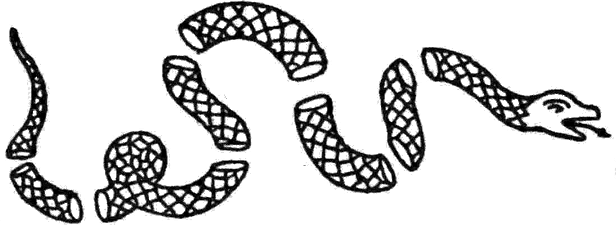
\includegraphics{join2.png}}
  % \rput[l](0,-4.5){\psscaleboxto(\textwidth,2){Speaking Serial R with a Parallel Accent}}
  % \rput[l](0,-4.5){\psscaleboxto(\textwidth,1.7){Speaking Serial R with a Parallel}}
  % \rput[l](6.0,-6.8){\psscaleboxto(4.3,1.7){Accent} \LARGE(Ver. \demoversion)}
   \rput[l](0,-4.5){\psscaleboxto(\textwidth,1.5){\Huge Speaking Serial R with a Parallel Accent}}
\end{pspicture}

\vfill\noindent
\ \hfill {\large\textsl{\pbdR Core Team}}
\end{document}
